% \setchapterstyle{kao}
\setchapterimage[6.5cm]{industry_1}
\setchapterpreamble[u]{\margintoc}
\chapter[机械幻想和智慧工厂:工业4.0]{机械幻想和智慧工厂:工业4.0\footnotemark[0]}

\footnotetext{The credits for the image above the chapter title go to:
	Image generated by OpenAI's DALL-E, used in accordance with OpenAI's terms and conditions.}


\section{引言}

创新是引领发展的第一动力。2013年德国政府提出“工业4.0”战略,并在当年的汉诺威工业博览会上正式推出。工业4.0指利用人工智能技术,由集中式控制向分散式增强型控制的基本模式转变,目标是建立一个高度灵活的个性化和数字化的产品与服务的生产模式。主要分为智能工厂,智能生产,智能物流三大主题。自提出以来,工业4.0迅速成为德国的另一个标签,并在全球范围内引发了新一轮的工业转型竞赛。

人工智能智慧工厂是工业4.0的核心主题之一。智慧工厂是指利用人工智能技术,辅助以大数据分析,多模态感知等先进技术手段,将传统工厂严重依赖于人工监督的流水线转变为智能化、自动化、高度灵活的生产方式。智慧工厂依赖于传感器、机器人、自动化设备和互联网等技术,实现生产过程的自动化控制、智能优化和数据驱动决策。在人工智能智慧工厂中,各种设备和系统可以相互连接和通信,形成一个智能化的生产网络。传感器和物联网技术能够实时收集和传输大量的生产数据,而人工智能算法则能够对这些数据进行分析和解读,从中提取有价值的信息。这些信息可以用于优化生产计划、预测设备故障、改进产品设计等方面,从而提高生产效率和产品质量。

如果说智能工厂改变了传统生产加工方式的执行者,那么智能生产则是统筹规划工业进程的指挥者。智能生产主要涉及整个企业的生产物流管理、人机互动以及3D技术在工业生产过程中的应用等。该计划将特别注重吸引中小企业参与,力图使中小企业成为新一代智能化生产技术的使用者和受益者,同时也成为先进工业生产技术的创造者和供应者。智能生产的概念涵盖了从生产计划、物料采购、生产过程监控到产品质量管理等方方面面,旨在构建一个高效、智能和可持续的工业生产体系。

智能物流是工业4.0的另一个主题。智能物流主要通过互联网、物联网、物流网,整合物流资源,充分发挥现有物流资源供应方的效率,而需求方,则能够快速获得服务匹配,得到物流支持。得益于我国巨大的消费市场,物流行业在我国有着广阔的发展前景。早在2008年,全国社会物流总额达89.9万亿元,比2000年增长4.2倍,年均增长23\%,较欧美发大国间同期领先200\%。中国物流与采购联合会发布的2023年物流运行情况分析指出,2023年全国社会物流总额为352.4万亿元,按可比价格计算,同比增长5.2\%,增速比2022年提高1.8个百分点,仍然占据着全球前列。我国在物流的智能化道路上同样进展喜人,2019年,京东物流在北京“亚洲一号”建设并落成国内首个5G智能物流示范园区,它实现了5G 网络通信与物流应用的深度融合创新,带来了智能物流园区的数字化与智能化。目前,我国坐拥成熟的快递物流系统,实现了物流的数字化管控,在智能物流方面处于世界领先水平。

\begin{marginfigure}
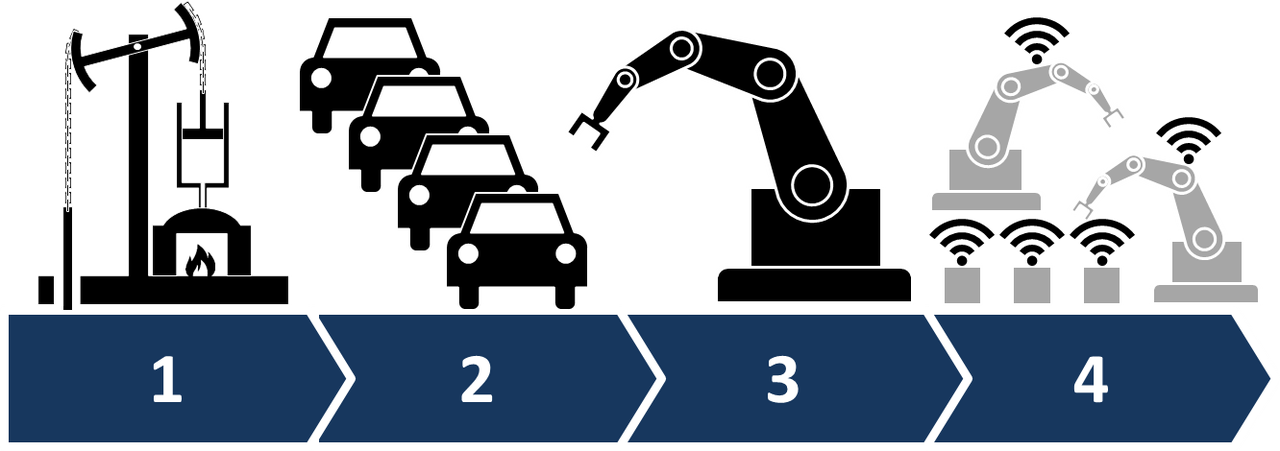
\includegraphics{images/industry_2.jpg}
\end{marginfigure}

自工业4.0提出以来,各国都开始了各自的工业改革道路,全球范围内展开了新一轮的工业转型竞赛。近年来,我国互联网企业发展迅速,人工智能技术在行业内应用逐渐成熟,已经为再一次产业升级打下了坚实的基础。我国政府对工业4.0保持了高度重视,早在2014年,我国就和德国签署了《中德合作行动纲要》。时任总理李克强表示:我国要在工业化与信息化同步发展的战略中更快地促进两者的融合。2015年,我国提出了《中国制造2025》的发展纲要,明确指出工业发展三步走的战略目标,即:到2025年,我国装备制造业进入世界装备制造强国第二方阵,部分优势产业率先实现又大又强;到2035年,我国装备制造业位居世界第二方阵前列,成为名副其实的装备制造业强国;到2045年,我国装备制造业进入世界装备制造强国第一方阵,成为具有全球影响力的装备制造业强国。2016年以来,诸多工业4.0相关政策陆续出台,包括《智能制造发展规划(2016-2020年)》、《智能制造工程实施指南(2016-2020年)》、《工业互联网创新发展行动计划(2021-2023年)等重磅政策陆续出台,从政策层面给予工业4.0重要的支持,更明确了我国工业4.0的发展目标及策略。与此同时,德国、日本、美国等制造业强国也都提出了各自的工业发展规划。可以预见的是,未来20到40年内,第四次工业革命将改变目前的生产生活方式,并且极大的影响着世界发展格局。

\section[机器人技术]{机器人技术:AI赋予机器自主行动能力}
\subsection{从“机器”到“人”,AI赋予机器新活力}

\begin{marginfigure}
    
\includegraphics{images/industry_3.jpg}
\end{marginfigure}

以机器代人工作的思想起源于文明发展初期,传闻春秋时期的工匠鲁班利用竹子和木料制造出一个木鸟,它能在空中飞行,“三日不下”,这件事在古书《墨经》中有所记载,可见人们对能够解放人类双手的生产方式渴望已久。1920年,捷克斯洛伐克剧作家卡雷尔·凯培克在他的科幻情节剧《罗萨姆的万能机器人》中,第一次提出了“机器人” (Robot)这个名词,被认为是机器人一词的起源。在捷克语中,Robot这个词是指一个服役的奴隶。这也是现在我们对机器人的一般理解,即能够帮助人类完成指定任务的机器。

通常将机器人发展历程分为三个阶段。第一阶段是可编程机器人,这类机器人通过人工编写的特定执行命令,不能根据环境调整自身行为,只能完成一些简单的重复劳作。第二阶段在可编程机器人的基础上添加了传感器,即自适应机器人。第二代机器人具有不同程度的感知能力,能够根据环境中特定指标的变化改变策略,目前大量应用于工业生产中。第三代机器人通过内置的人工智能程序进行调度,具有识别、推理、规划和学习等智能机制,它可以把感知和行动智能化结合起来,因此能在非特定的环境下作业,故称之为智能机器人。

人工智能技术使得机器人真正跳出了预设的框架,迈向了智能化,自主化的新阶段。下面我们来介绍人工智能用于机器人的几个关键技术。

感知与认知技术是人工智能机器人的关键技术之一。以各类传感器为基础,感知技术为机器人提供了观测实际环境的能力。机器人可以从环境中获取各种传感器数据,如视觉、声音、温度、磁场等信息,并立即进行处理和分析,转化为机器人能够理解的数据流。随后,以数据挖掘,深度学习,强化学习等智能算法为核心的认知技术对感知得来的数据进行理解和解释,通过学习和推理来做出智能决策和行为。要将感知学习与认知科学结合起来并非易事,如何面对复杂多变的真实情况是机器人技术难以绕开的问题。为此,研究人员搜集整理了大量实际生产中的数据,包括各种情况下恰当的做法,这部分也称为“记忆”,用于训练模型,由此来理解和推理实体物质。在构造好适宜的数据后,深度学习和强化学习彼此构建,形成了一种强有力的人工智能开发方式。深度学习能够处理各类型的数据,允许计算机解决更加复杂深奥的任务,包括视频、图片理解和语音处理等;而强化学习模仿了人类的学习过程,引进了奖励/惩罚机制对机器人的每个动作进行评估,从而引导机器人做出正确决策,获得长期收益。目前,感知与认知技术已经在自动导航,故障监测,智能控制等方面得到广发运用,并取得巨大的成功。

人机交互与自然语言处理技术是增强人机沟通和互动的重要技术。通过设计用户友好的界面和自然易懂的交互方式,如语言指令、手势识别和面部表情识别,人与机器人之间可以进行高效、透明的交流。自然语言处理技术旨在研究人类和机器之间用自然语言进行有效通信的理论和方法。自然语言处理技术的发展,意味着人们可以使用熟悉的语言对计算机下达指令,而不需要学习复杂的编程语言,体现出现代计算机技术面对大众的特点。在实际应用中,智能机器人需要面对不具备编程能力的用户,自然语言处理技术使二者的交互更加高效。自然语言处理技术来源于条件概率,计算机首先对大量的语言进行处理,从而学习到给定上下文的情况下,特定位置应该是哪些单词,从而构造出一个自然语言处理模型。在使用过程中,模型将用户问题输入为上文,基于条件概率预测下文中概率最大的内容,作为对用户问题的回答。随着全球经济下行和人力成本的上涨,以服务业为首的部分第三产业遭受了严重的冲击,服务机器人的需求进一步增加。搭载了自然语言处理模型的机器人能够面对用户不同的问题,同时通过各类接口,机器人可以用作不同功能的集成终端,进一步减少工业、服务业的人工与管理成本。服务机器人已经在银行,餐馆,展览等需要大量人工服务与交互的行业投入使用。随着GPT系列模型在自然语言、计算机视觉、工具调用等领域取得的巨大成功,未来的服务型智能机器人将获得进一步的发展。

多机器人协作与协同技术具有广阔的应用前景。通过智能任务分配的和协同决策算法,多个机器人、人与机器人可以在不同任务和环境中实现高效的协作工作。在协作机器人技术中,协同控制是指多台机器人在工作时,通过共享信息和协同调度来达到高效率,高稳定性和高性能的工作状态。一般来说,机器人组进行协同的方式有两种:集中式决策与分布式决策。集中式决策将所有决策任务分配给中心节点,其负责所有机器人的任务分配和协同控制,其他机器人只负责执行任务。集中式方法适合任务相对简单,机器人之间的通信成本均较低的任务。而分布式算法中,每个机器人都会具有一定的决策能力,能够根据自身附近的环境进行决策。分布式决策适用于任务复杂,机器人之间通信成本较高的任务。多机器人协作任务不仅需要机器人规划自己的行为,还需要及时将自身信息发送出去,方便与其他机器人协调,对计算机的性能有着较高的要求,也在一定程度上限制了复杂的协作机器人的落地应用。目前只有自动运输领域使用多机器人协作技术进行调节与规划,仍然存在不少问题需要解决。

\subsection{从“人”到“机器”,机器人技术的发展与应用}

1958年,被誉为“工业机器人之父”的Joseph F.Engel Berger创建了世界上第一个机器人公司——Unimation(Univeral Automation)公司,并参与设计了第一台Unimate机器人,用于机器间的物料运输。自此之后,工业机器人进入蓬勃发展时期,并且快速迭代到了第二代感知机器人。与此同时,日本,欧洲等国家也意识到了工业机器人的发展潜力,并加大了研发力度,智能机器人的雏形也诞生于这个阶段。经过20余年的蓬勃发展,工业机器人已经在大规模生产和制造中占据主流地位。直到80年代后期,由于传统工业机器人市场已经进入饱和,计算机与人工智能领域发展停滞,机器人产业出现不景气。进入21世纪以来,得益于智能算法的快速发展,机器人行业出现复苏和快速发展迹象。直到今天,人工智能呈井喷式发展,智能机器人的研发和生产逐渐取代了感知机器人,引领了又一轮机器人行业的快速发展。

\begin{marginfigure}
    
\includegraphics{images/industry_4.JPEG}
\end{marginfigure}

我国是从二十世纪八十年代开始机器人的研究和应用的。“七五”计划提出了机器人发展战略,明确指出要将机器人领域的发展作为重点工作。得益于广阔的市场和丰富的原材料,自2007年至2020年,我国机器人产业生产总值年均增速500\%,远超欧美等发达国家。2023年,深圳市机器人产业营收超过1700亿,位于世界前列。目前,我国机器人行业已经形成了企业主导,政策扶持,市场检验的发展模式,不断推动我国工业4.0的升级换代。其中以埃斯顿,科沃斯,新松等龙头企业最为突出。下面以新松机器人的发展情况为例,介绍我国机器人企业的发展历史,业务范围和研发展方向。

沈阳新松机器人成立于2000年,主营业务以机器人技术和智能制造解决方案为核心,以智能制造为业务主攻方向,并成为了国家级机器人产业化基地,并在中国机器人行业标准制定中发挥了关键作用 ,目前位列中国机器人协会会长单位。另一方面,新松积极布局国际市场,在世界各地设立海外分子公司及区域中心,产品累计出口至全球40多个国家和地区。

新松机器人主营产品包括工业机器人,移动机器人,特种机器人,协作机器人几大类。工业机器人以机械臂为主,已经具备智能感知、智能认知、自主决策、自控执行等功能,能够在一定程度上自动化处理生产中出现的问题;移动机器人包括扫地机器人,运输机器人等,具有自动寻路,自动避障,实时决策等功能;特种机器人包括探测机器人,应急机器人,为应对各种突发情况;协作机器人已经实现了与人工合作,在防爆,精密控制等方面有着突出的贡献。除此之外,新松机器人还涵盖了医疗、生产、交通等多个方面。

中国机器人行业虽然起步较晚,但是得益于我国在制度、市场等多方面的优势,目前我国机器人行业规模位于世界领先地位。但是还需要注意,我国在高精尖的技术方面和欧美等发达国家仍有一定差距,在算法领域还处于落后地位。随着大模型技术展现出强大的能力,新一轮的基于已经到来,未来阶段,大模型在机器人的动作预测,人机交互,指令遵循等方面将有着广泛的运用。

\section[生产流程优化与质量控制]{生产流程优化与质量控制:AI提高生产效率和质量}
在当今快速发展的制造业中,企业面临着提高生产效率和质量的巨大挑战。生产流程的优化和质量控制成为企业取得竞争优势和提高利润的重要手段。然而,传统的生产流程和质量控制方法往往面临着许多限制和挑战,包括人工操作的局限性、数据分析的复杂性以及应对变化和不确定性的能力。智慧工厂作为工业4.0的核心内容,采用人工智能辅助,为传统的生产流程控制和产品质量优化带来了革命性的变革。AI的强大计算能力和智能算法使得企业能够更加全面、准确地监测和分析生产过程中的关键数据,从而实现实时的生产过程优化和质量控制。除此之外,AI还能够自动化决策和调整,降低人为错误的风险。

本章将探讨AI在生产流程优化和质量控制方面的应用。首先,我们将探讨AI在生产过程优化中的应用,包括智能调度、自动化控制和预测性维护。最后,我们将研究AI在质量控制和缺陷检测方面的应用,包括图像识别、机器学习和自动化检测技术。通过充分利用AI的优势,企业可以实现更高效、更灵活和更智能的生产方式,迈向智能制造的新时代。

\subsection{从原料到成品:AI控制下的生产流程}
在上一章中,我们介绍了规格不同,功能各异的智能生产机器人。通过预编程与训练,机器人可以完成一系列指令,从而将送入的材料加工为成品。人工智能对机器人技术的发展迭代起到了决定性的作用。然而,人工智能技术在智能工厂中起到的作用远不止于此。除开对每个特定的机器人进行控制以外,以智能规划为主的人工智能算法还能对整个工厂的生产过程进行规划和指导。以一个普通的工厂为例,从原材料到成品需要经过“从厂外运输-加工为半成品-厂内运输-加工为成品-输出工厂”的流程。传统方法需要由人对其中各个环节进行调度,包括原材料的消耗量,成品的销售量,运势所需的路线和时间等等。然而使用人工智能进行辅助的智慧工厂可以实现全流程。

\begin{marginfigure}
    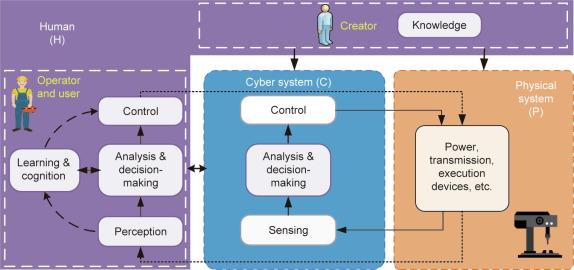
\includegraphics{images/industry_5.jpg}
\end{marginfigure}

生产计划是制造业中至关重要的环节,它涉及到资源分配、任务调度、交货期管理等方面。由于人工处理信息具有滞后性和易错性,传统工厂对生产计划很少进行修改,修改所需的时间通常以季度为单位,经常导致工厂的生产量难以对市场的迅速变化做出反应。人工智能(AI)技术在生产计划方面的应用可以帮助企业实现更准确、高效和灵活的计划,从而提高生产效率和降低成本。时间序列分析是制定生产计划时常用的技术之一。一般来说,商品的需求量受到时间的影响,在整体趋势上呈现季节性变化。但是,当多种影响因素综合时,商品的需求量变化将变得难以预测。时间序列分析算法目标是将季节性变化与回归分析结合起来,将需求量随时间的变化趋势拆解为多个与时间强相关的变量,从而对未来走向进行预测。与人工方法相比,时间序列分析算法能在更高的维度上对数据进行处理,从复杂变化中寻找规律的能力更强,并且有着更快的反应速度。目前时间序列分析已经在电力,水利等多个产业投入使用,利用大数据分析和机器学习算法对历史生产数据进行挖掘和分析,以识别潜在的模式和趋势。通过对市场需求、供应链状况和生产能力等数据的综合分析,提供准确的预测和需求预测,帮助企业做出更合理的生产计划。

运输被称为工业的血液,它在整个供应链中扮演着运转枢纽的角色。运输的效率和质量直接影响到生产计划的执行和产品的交付。为了实现高效的运输管理,人工智能技术被广泛应用于物流和运输领域。人工智能的应用使得运输过程更加智能化、可优化,并带来了许多优势和创新。一般来说,智能工厂采用蚁群算法对多个物品的运输路线进行规划。蚁群算法属于演化算法的一种,通过模拟蚂蚁在搜索过程中释放信息素的行为,算法可以自适应地调整蚂蚁的移动方向和路径选择,以实现多个物体的有效运输路线规划。除了路线的规划,人工智能技术结合物联网技术,可以实时追踪货物的位置、运输条件和运输状态。这使得企业能够及时了解货物的运输情况,并及时采取调整措施,以确保货物的安全和交付准时。

\subsection{保质保量,生产安全:AI的质量检测和安全保证}
对于工业4.0,工业安全和质量控制是两个至关重要的方面,对于企业的可持续发展和生产运营的稳定性具有重要意义。进入工业4.0时代,随着计算机视觉与多模态技术的发展,这两个方面也迎来了翻天覆地的变化。

\begin{marginfigure}
    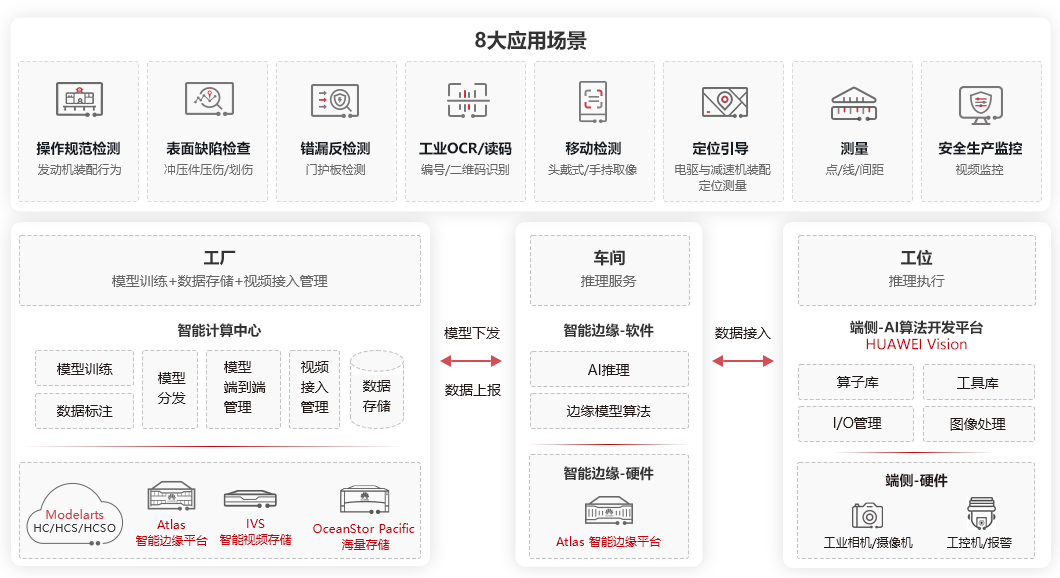
\includegraphics{images/industry_6.png}
\end{marginfigure}

工业安全一直是企业关注的焦点,因为安全事故可能导致人员伤亡、设备损坏和生产中断。一直以来,工厂的故障检测都依赖于人力巡查,这不仅对工人的素质有着极高的要求,还需要大量的人力物力资源。进入工业4.0时代后,工厂大采取了综合多样数据的安全检测系统,助企业及时识别安全风险和潜在危险,从而采取预防措施并减少事故发生的可能性。例如,通过使用智能传感器和视频监控系统,AI可以实时监测生产现场的温度、压力、气体浓度等参数,并识别异常情况。同时,基于机器学习和模式识别算法,AI还可以分析历史数据,发现隐含的安全风险,并提供决策支持,促进企业的安全管理和风险控制。

质量控制是确保产品符合规格和客户需求的关键环节。原本的质量检测方式基于采样检查,需要在成品中进行随机抽取,通过概率分布计算整体的次品率。然而,这样的方法有以下几个缺点:首先,如果次品率不达标,那么这批产品都需要重新生产,会造成巨大的资源浪费;其次,人工检测会受到主观因素影响,可能会导致用户差评。目前的人工智能技术可以在生产途中对产品质量进行检测,通过视觉模块和传感器,对产品次品率进行实时计算。当次品率升高时,机器可以实时调整策略,或者向检测人员报警,从而提高生产质量,避免因次品率高导致的资源浪费。 

\subsection{实践真知:我国工业4.0流水线发展现状}

\begin{marginfigure}
    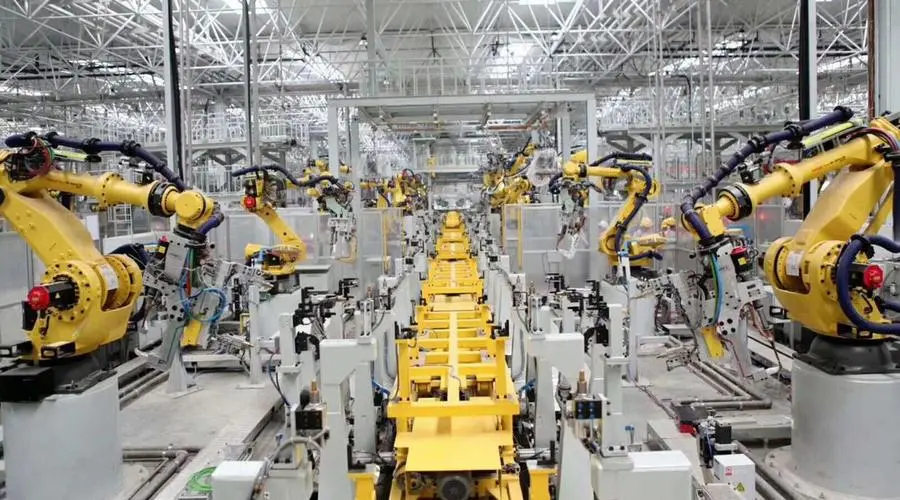
\includegraphics{images/industry_7.png}
\end{marginfigure}

目前,人工智能控制下,集成生产,监测,运输的多功能流水线已经趋于成熟,我国的也已经有较多企业采取了这样的生产方法。汽车行业包含了钢铁铸造,橡胶生产,精密仪器制造和整体加工组装等多个方面,需要一套完备可靠的调度系统对整个生产线进行规划。比亚迪(BYD)是中国领先的新能源汽车制造商和技术解决方案提供商,其自动生产运输流水线是其制造业务中的重要环节。比亚迪的自动生产运输流水线是一种高度自动化和智能化的生产系统,旨在提高生产效率、降低成本并确保产品质量。该流水线采用了先进的物联网和人工智能技术,实现了从零部件生产到最终组装的端到端自动化。

在比亚迪的自动生产运输流水线中,各个生产环节都经过精心规划和优化。首先,原材料和零部件的供应链被整合到系统中,通过物联网技术实现了供应链的实时监控和管理,确保零部件的及时供应和库存控制。

生产方面,比亚迪的自动化生产线利用机器人、自动化设备和传感器等技术,对零部件进行加工和组装。这些设备能够高效地完成各种工序,如焊接、喷涂、装配等,减少了人工操作的需求,提高了生产效率和一致性。

在运输环节,比亚迪采用了自动导引车(AGV)和无人驾驶车辆(AV)等技术,实现了物料和半成品的自动运输。这些智能车辆能够根据生产计划和物料需求,自动识别和获取所需物料,并将其运送到相应的生产线或工作站。通过使用自动运输系统,比亚迪能够减少人力投入和物料损耗,提高运输效率和准确性。

整个自动生产运输流水线通过物联网技术实现了各个环节的数据收集和监控。传感器和监测设备可以实时获取生产数据,并将其传输到中央控制系统进行分析和优化。这使得比亚迪能够实现实时生产监控、故障诊断和预测性维护,提高生产线的稳定性和可靠性。
比亚迪的自动生产运输流水线不仅在新能源汽车制造领域取得了显著成就,还在其他行业中得到了广泛应用。其高度自动化和智能化的特点使得生产过程更加高效、可控和可持续,为企业实现数字化转型和智能制造提供了有力支持。



\section[供应链管理]{供应链管理:AI实现需求与库存管理}

\subsection{智慧仓库变革史}
除生产方式的变革之外,工业4.0还带来了供应链管理方面的进步。供应链管理是一个复杂而关键的领域,涉及到了多个环节和各种资源的协调与管理。在过去,供应链管理往往依赖于人工智能以外的手段和经验,这导致了一些挑战和限制。然而,随着人工智能技术的快速发展和应用,供应链管理正迎来一场革命性的变革。

\begin{marginfigure}
    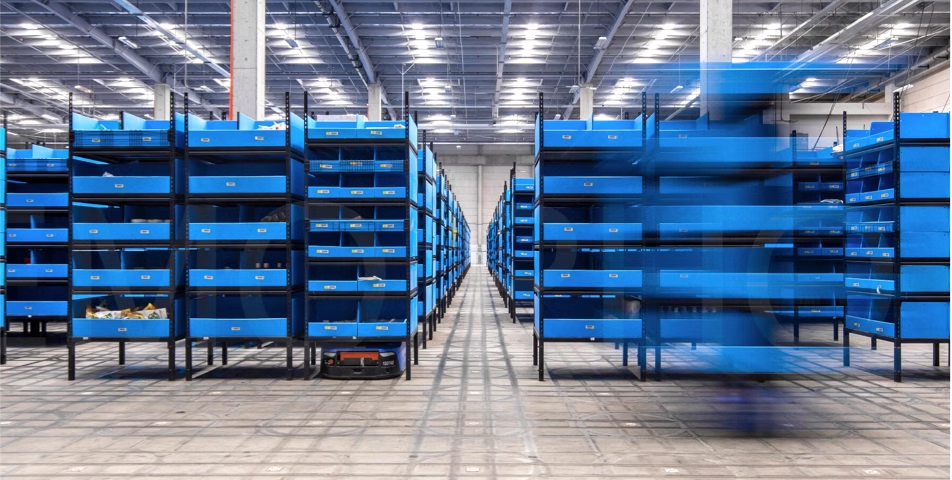
\includegraphics{images/industry_8.png}
\end{marginfigure}

人工智能在供应链管理中的应用已经展现出了巨大的潜力,特别是在需求与库存管理方面。传统的需求与库存管理常常受限于不准确的预测和缺乏实时信息的问题,导致了过剩库存或缺货的情况。而人工智能技术可以通过数据分析、机器学习和优化算法等手段,实现更精准、高效的需求与库存管理。本章节将探讨人工智能在需求与库存管理中的应用,以及它所带来的优势和挑战。

库存管理包括物品的流入与流出,实时检测库存量和剩余容量,对未来一段时间内的容量变化的预测等方面。在人类历史上,早在早期农业时代就有仓库的概念了,当时人们使用结绳或是刻画的方式对仓库内粮食的数量进行记录,间接推动了文字和数学的发展。进入封建时代,对粮食的管理和控制成为农业社会的重点,封建朝廷也设立了各级官吏对粮仓进行管理。粮官使用账本对粮食的进入和流出进行记录,但是这样的方法有着不小的问题:首先,使用人工记录的方法容易出现主观或客观的错误,为了避免贪腐问题的出现,封建社会采取了多级监管的机制,但是收效甚微,反而导致了官员冗杂的问题;其次,原始的管理方式难以对库存需求进行预测,存储商品所需的开销往往是巨大的,长时间的存储不仅会增加商品损坏的几率,还会浪费大量的资源。进入新时代以来,计算机技术的发展为管理提供了新方式,使用计算机进行库存计算避免了客观失误带来的错误,却还是没能解决库存预测,动态调整等问题。直到人工智能技术的发展与工业4.0的变革出现,库存管理方式才解决了长久以来的问题。

人工智能可以分析大量的供应数据和实时销售信息,实现对库存水平的动态监控和优化。通过智能算法和模型,企业可以根据需求变化和供应能力进行库存的合理分配和调整,确保库存水平在经济性和服务水平之间达到最佳平衡。这有助于减少库存成本、提高资金利用率,并确保及时满足客户需求。人工智能的预测功能保证了每次库存都能满足需求,同时不会过多,避免了因过度囤积导致的浪费。

\subsection{动态平衡供应链}

除了库存问题,供应链也是物联网中至关重要的部分。供应链是指涉及从原材料供应商到最终客户的物流和商务活动的网络。一个稳定运行的供应链不仅包含从生产地运送到目的地这样简单的工作,还包括了数量充足的出货仓库,损耗最小的运输方式,路程最短的运输路线等多个问题,使用了动态规划,最优路径搜索,回归分析等多种算法,在供应链管理中的应用可以提供更智能、高效和可靠的解决方案,优化运营效率、降低成本,并提供更好的客户体验。

首先,人工智能可以帮助企业在众多供应商中选择最佳的合作伙伴。通过分析供应商的绩效数据、信用评级和交付能力等因素,人工智能可以提供客观、数据驱动的供应商选择和评估指标,帮助企业做出更明智的供应商决策。此外,人工智能还可以监测供应商的交付状态和质量表现,提供实时的供应商绩效评估和管理支持。

其次,人工智能可以通过模拟来选择最优的运输路线,在存在多个发货地和多个目的地时,人工方法很难寻找到一个最优的运输规划。相对的,通过分析运输数据、交通状况和运输需求等信息,优化物流和运输计划。人工智能可以帮助企业选择最佳的运输路径和模式,提供实时的货运跟踪和交通调度,减少运输时间和成本,并提高交货准时率。人工智能采取遗传算法解决运输规划问题,通过在模拟环境中不断迭代,从而找到一个最优的规划,极大的减少了错误规划的可能性,避免了资源浪费。

最后,人工智能可以帮助企业识别和管理供应链中的风险因素。由于人工检测需要大量专业员工实时监控,并且严重依赖于各基层的检测结果,对整个供应链的监测力度不够。并且单纯的监测系统不能提供风险预测与评估。通过分析供应链数据和外部环境信息,人工智能可以提供风险预警和应对措施,帮助企业更好地应对供应中断、自然灾害、市场波动和质量问题等风险。

\subsection{供应与库存:领先世界的快递业}
中国的快递业是全球最大、最发达的快递市场之一。随着中国经济的快速增长和电子商务的兴起,快递业在过去几十年中蓬勃发展,成为中国物流行业的重要组成部分。中国的快递业得益于电子商务的强大推动力,自2000年以来,中国的电子商务迅速发展,成长为全球最大的电子商务市场之一,众多的电商平台和在线零售商的崛起促使了快递服务的需求迅速增长。消费者可以通过网上购物轻松购买商品,并通过快递服务便捷地将商品送到家门口。同时,为了应对快递业务的快速增长,中国的快递业进行了大规模的基础设施建设。快递企业建立了庞大的分拣中心、配送中心和仓储设施,投资大量资金用于信息技术和物流设备的更新和升级。这些投资提高了物流效率和服务质量。市场需求与政府扶持的双重推动下,中国的快递业积极探索科技创新,引入人工智能、大数据分析、无人机、机器人等先进技术,以提升业务效率和服务质量。目前已经成为全球最大的快递业市场。

中国的电商企业目前由京东和阿里巴巴领跑。除了因为这两个电商平台包含商品种类多样,物美价廉之外,还得益于二者在物流业上的布局。中国的制造业大多集中在东南方沿海地区,全国的大部分订单都由这里发货。但是由于中国广阔的地理面积,向西部和北部进行运输需要极大的时间与资源开销。为了解决这个问题,中通、圆通等快递公司与淘宝达成合作,为淘宝商户提供较低的收费。另一方面,快递公司对每件商品进行独特的编码,使用人工智能技术选择最优的运输路线,并且实时将物流信息同步给客户,为客户提供良好的快递体验。与之相对的,京东拥有自己的快递业务,京东在中国大部分主要城市都有仓库,通过智能化的管理,可以对仓库内库存进行动态管理,以满足各地的货物需求,从而达到更快的运输效率。